\documentclass[letterpaper,12pt]{article}
\usepackage{tabularx} % extra features for tabular environment
\usepackage{amsmath}  % improve math presentation
\usepackage{float}
\usepackage{pdfpages}

\usepackage{multicol}
\usepackage{graphicx} % takes care of graphic including machinery
\graphicspath{ {./figures/} }
%\usepackage[margin=1in,letterpaper]{geometry} % decreases margins
%\usepackage{cite} % takes care of citations
\usepackage[final]{hyperref} % adds hyper links inside the generated pdf file
\hypersetup{
	colorlinks=true,       % false: boxed links; true: colored links
	linkcolor=blue,        % color of internal links
	citecolor=blue,        % color of links to bibliography
	filecolor=magenta,     % color of file links
	urlcolor =blue         
}
\usepackage[margin = 1in,headsep=0.5cm,headheight=2cm,letterpaper]{geometry} 

\usepackage{fancyhdr}
\pagestyle{fancy}
\lhead{Student 1 : Ahmet Akman 2442366 \\ Student 2: Yusuf Toprak Yıldıran 2444149 \\ Assistant: Onur Selim Kılıç}
\rhead{Date: \today \\ Group: Wednesday Morning - 5} 
%\cfoot{center of the footer!}
\renewcommand{\headrulewidth}{0.1pt}



\begin{document}
\thispagestyle{empty}

\title{Spring 2022 EE214 Experiment 6  \protect\\ Frequency Response}
\author{Ahmet Akman 2442366 \protect\\ Yusuf Toprak Yıldıran 2444149 \protect\\ Assistant: Onur Selim Kılıç}
\date{\today}
\maketitle
\tableofcontents
%\begin{abstract}
%abstract
%\end{abstract}
\section{Introduction}

\section{Experimental Results and Discussion}
The results of the experiment are discussed in the following steps.
%
\subsection{Step 1}
\subsubsection{a.}

\subsubsection{b.}

\subsection{Step 2}
In this step the circuit given in Figure X is constructed. The switch was kept open. 
\begin{figure}[H]
    \centering
    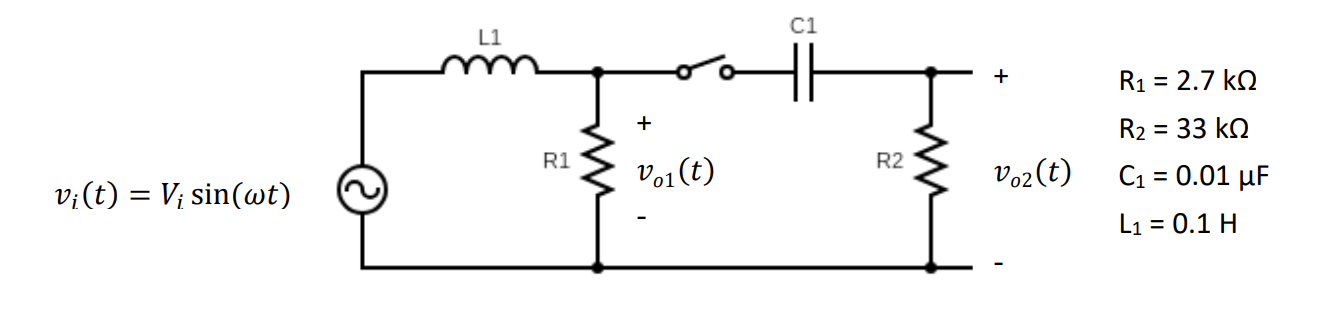
\includegraphics[width = 0.75\textwidth]{lowqlowpass.png}
    \caption{Circuit schematic for the step 2}
\end{figure} 
Then similar to the previous step, a test flow on the BenchVue is ran. Then the outputs of the test flow is exported as a MATLAB data file. The data is imported in MATLAB .The plots of phase response and magnitude response is plotted which are given in Figures X and X.
\begin{figure}[H]
    \centering
    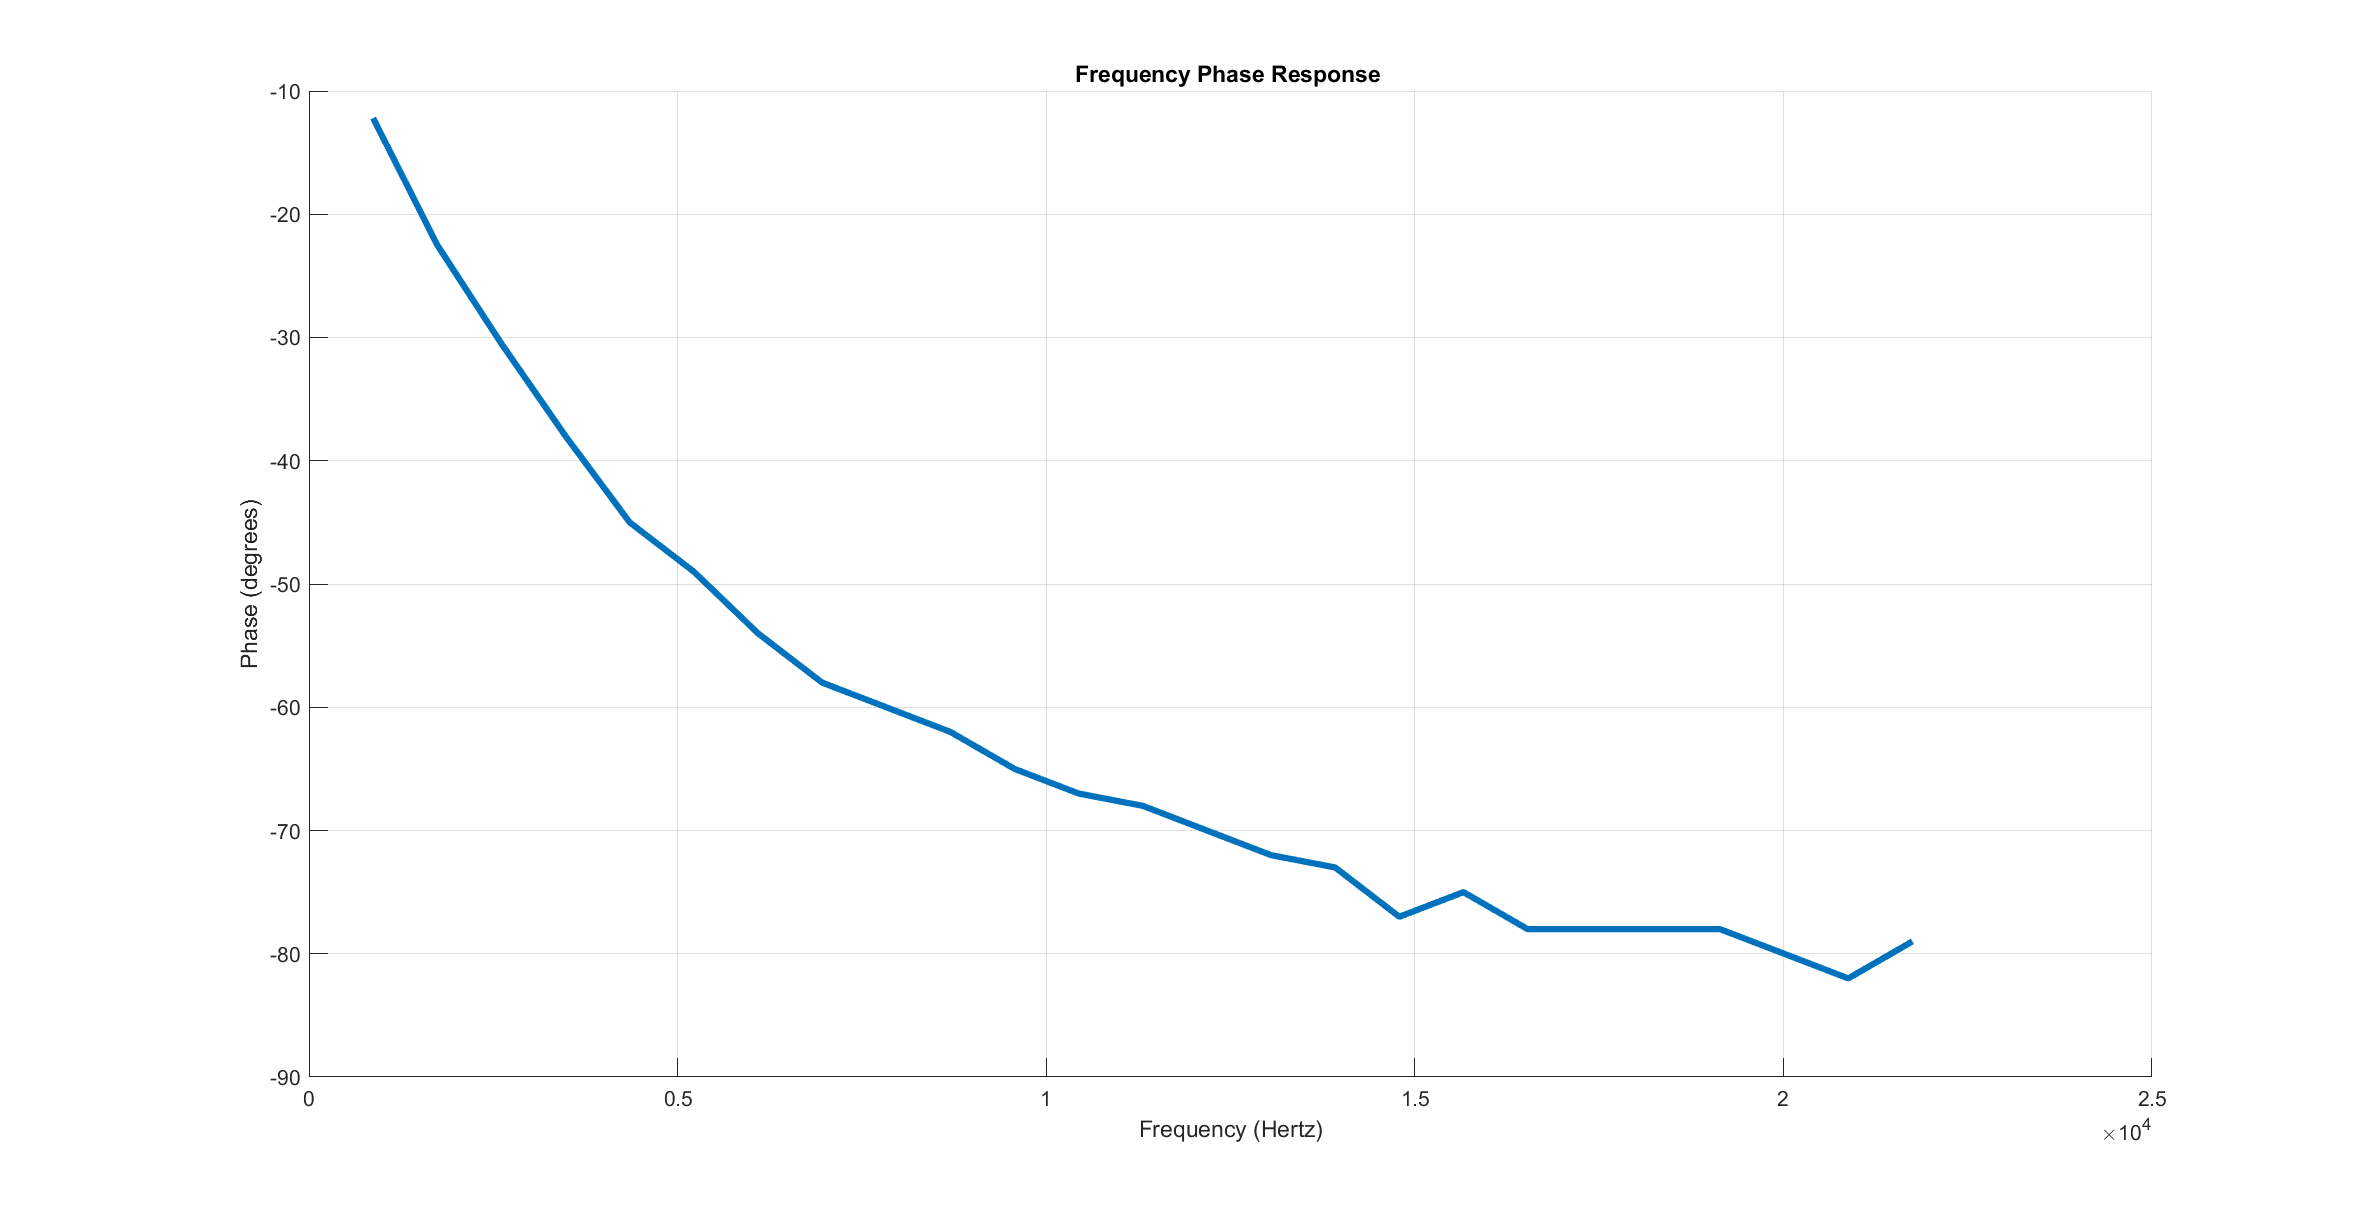
\includegraphics[width = 0.75\textwidth]{2_1_2.png}
    \caption{Phase Response of the Low-Q RLC filter.}
\end{figure} 

\begin{figure}[H]
    \centering
    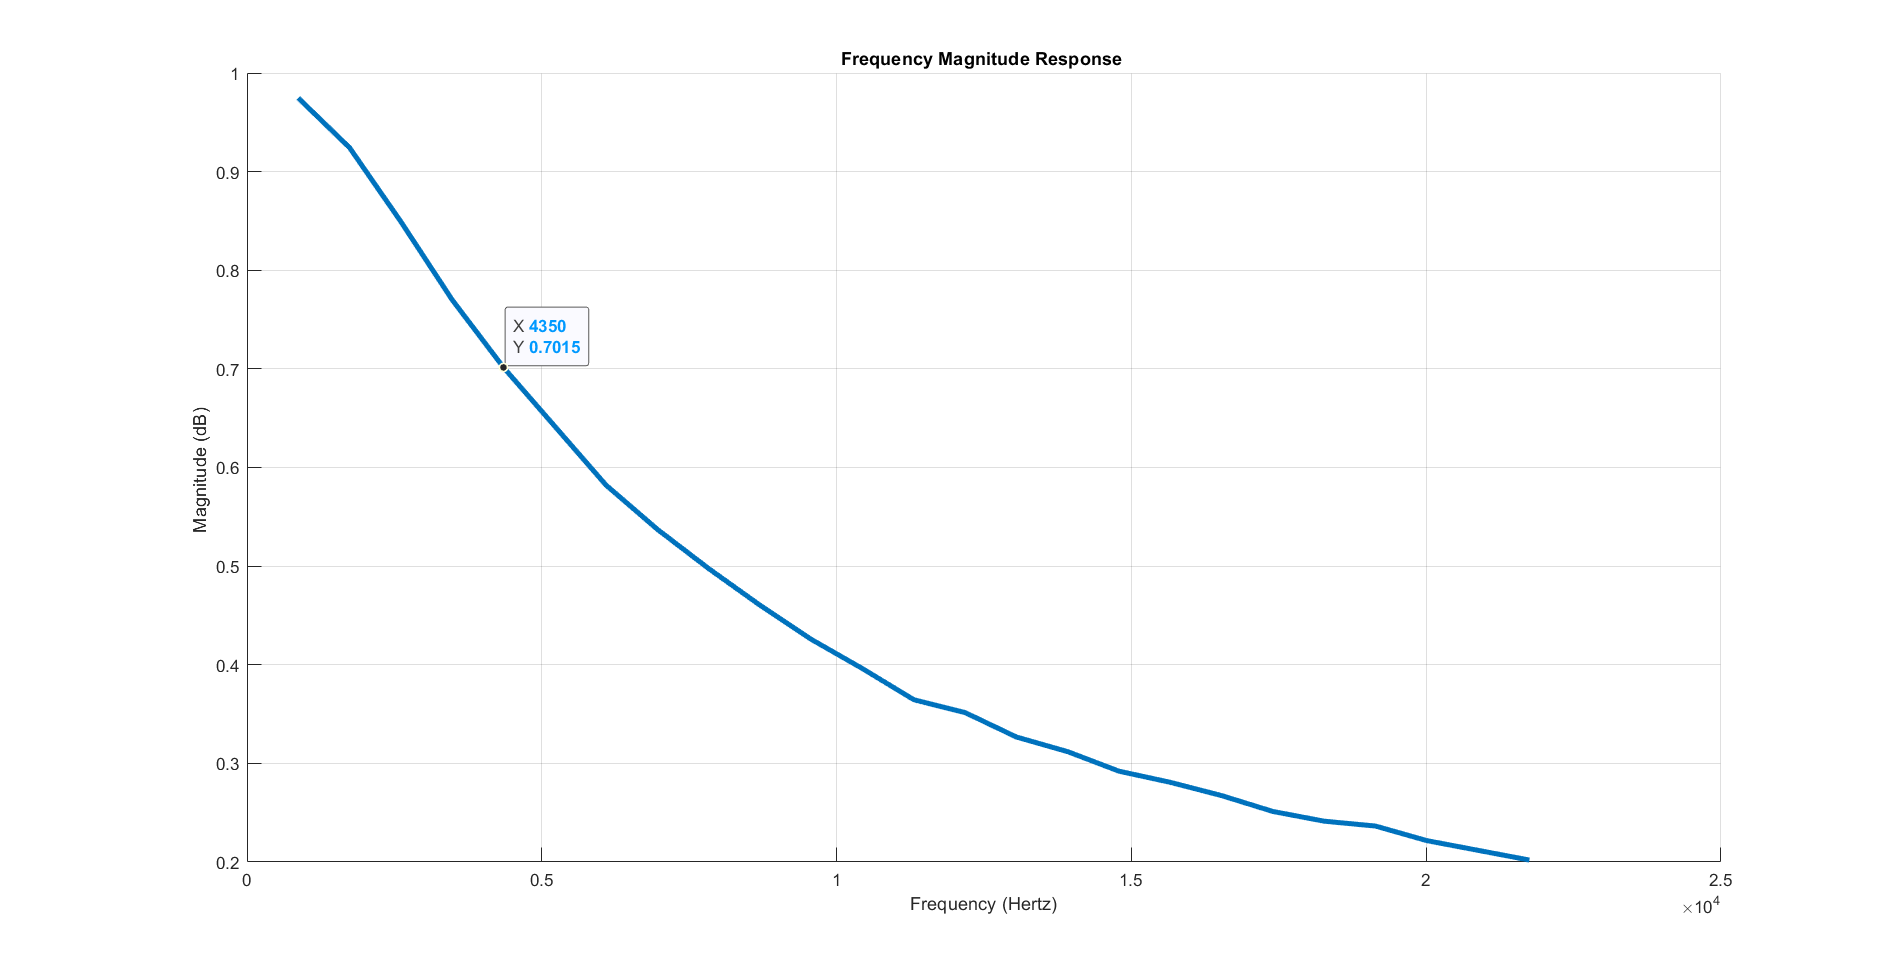
\includegraphics[width = 0.75\textwidth]{2_1_1.png}
    \caption{Magnitude Response of the Low-Q RLC filter.}
\end{figure} 
The value fo the \(\omega_c\) is pinned in the magnitude response plot. As a result it can be concluded that the circuit is an example of a passive low pass filter. Low pass filters allow only the frequencies below the thereshold.  By looking at the sharpness of the responses it can be said that the Q (the quality factor) of the circuit is low. 
    
\subsection{Step 3}
In this step the circuit given in Figure X is set on the breadboard. The C value is taken as 0.01\(\mu F\) as it was found in the preliminary work. 
\begin{figure}[H]
    \centering
    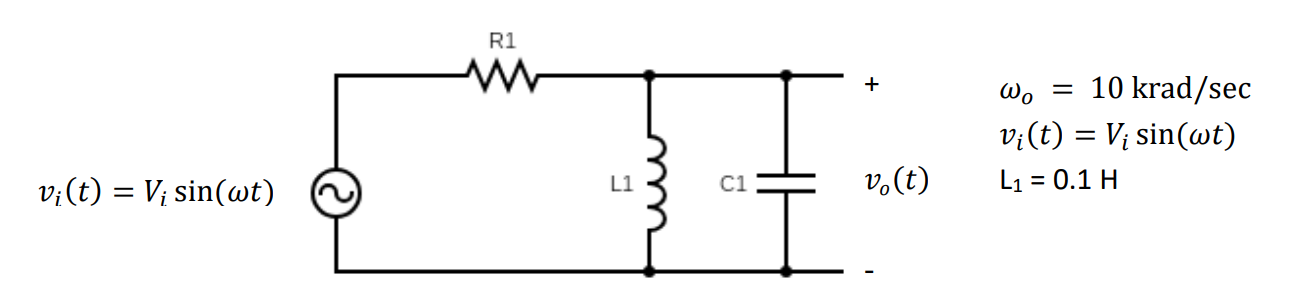
\includegraphics[width = 0.75\textwidth]{highqbandpass.png}
    \caption{Circuit schematic for the step 3}
\end{figure} 
Then similar to the previous steps the test flow on BenchVue is ran. As a result the magnitude and the phase responses given in Figures X and X are obtained. 
file. The data is imported in MATLAB .The plots of phase response and magnitude response is plotted which are given in Figures X and X.
\begin{figure}[H]
    \centering
    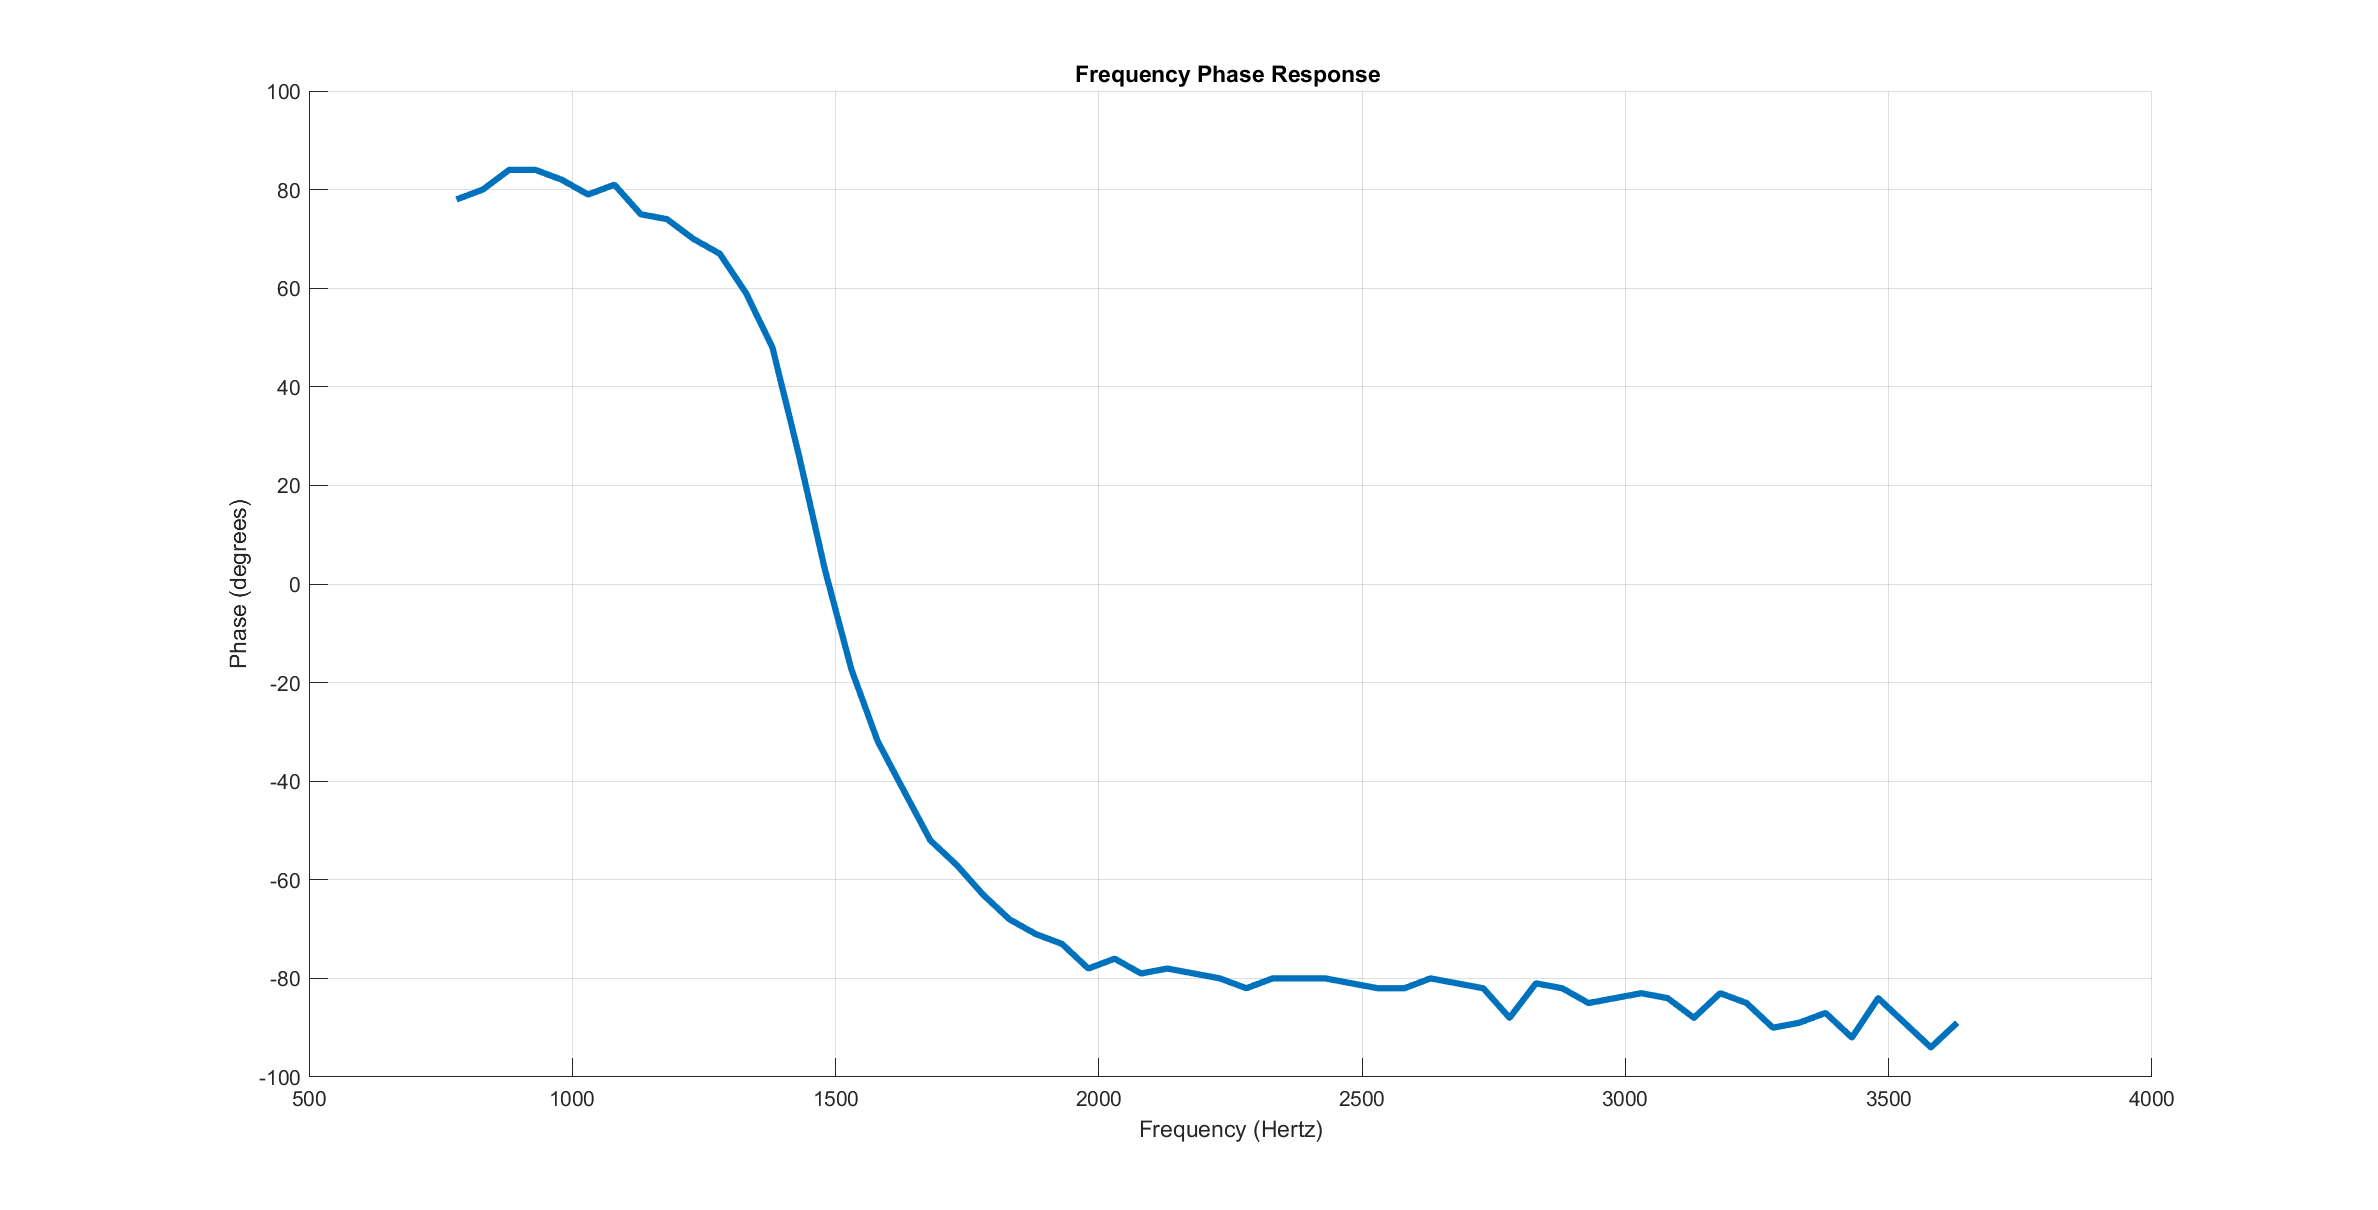
\includegraphics[width = 0.75\textwidth]{3_1_2.png}
    \caption{Phase Response of the High-Q RLC filter.}
\end{figure} 

\begin{figure}[H]
    \centering
    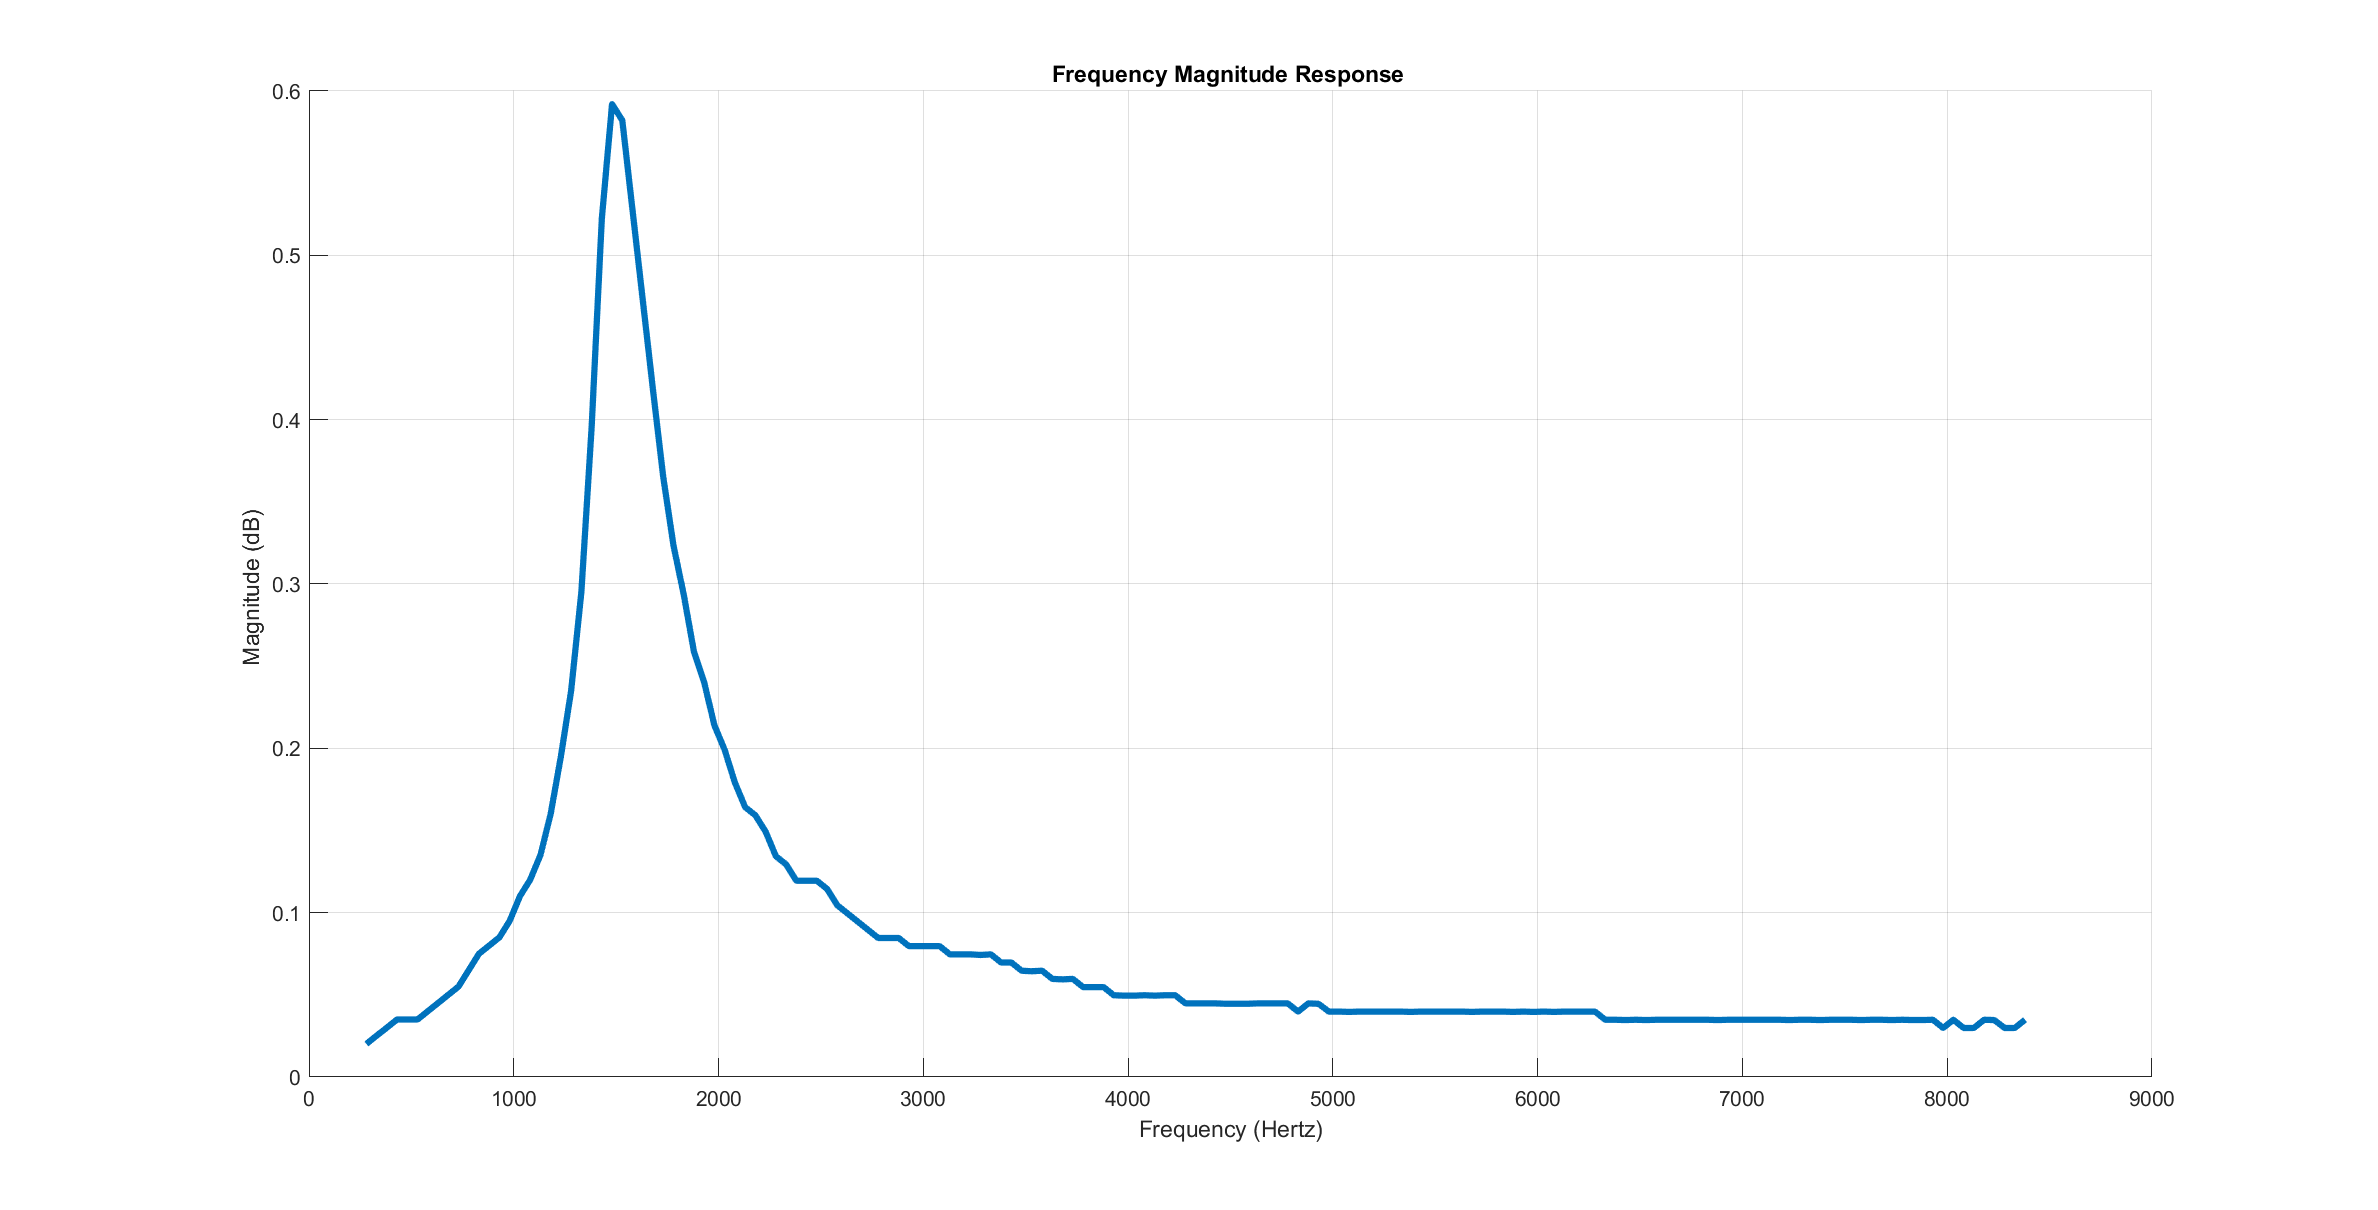
\includegraphics[width = 0.75\textwidth]{3_1_1.png}
    \caption{Magnitude Response of the High-Q RLC filter.}
\end{figure} 
The values \(\omega_{c1}\) ,\(\omega_{0}\) and \(\omega_{c2}\)  are indicated in the magnitude response plot with data pins. This filter is a band pass filter that only allows certain band of freqencies to pass on. The Q (Quality Factor) of the filter is calculated as 3.821 which can be consired as a high Q.  This also intuitively gives an idea on the sharpness of the phase angle plot.  

\subsection{Step 4}
\subsubsection{a.}

\subsubsection{b.}


\section{Conclusion}



\section*{Appendix A}
\begin{itemize}
    \item PreLab Preparation 3 hours
    \item Experimental Work 2  hours
    \item Report Writing 8 hours
\end{itemize}
\section*{Appendix B}
In this experiment, since the values the students obtained in the lab is quite close to the data provided by the lab assistants, it is preffered to use the data obtained by the students.

\end{document}

%%%%%%%%%%%%%%%%%%%%%%   EXAMPLE TABLE   %%%%%%%%%%%%%%%%%%%%%%%%%%%%%%%%
\begin{table}[H]
\begin{center}
    \caption{Resistance reading by color code convention.}
    \vspace{2mm}
    \begin{tabular}{||c | c | c||} 
        \hline
        Color Order & Value & Tolerance \\ [0.5ex] 
        \hline\hline
        Brown / Black / Red / Gold & 1k\( \Omega \) & \( \% \) 5  \\ 
        \hline
        Yellow / Violet / Red / Gold & 4.7k\( \Omega \) & \( \% \) 5   \\
        \hline
        Brown / Grey / Orange / Gold & 18k\( \Omega \) & \( \% \) 5  \\ [1ex] 
        \hline
    \end{tabular}
\end{center}
\end{table}


%%%%%%%%%%%%%%%%%%%%%%   EXAMPLE IMAGE   %%%%%%%%%%%%%%%%%%%%%%%%%%%%%%%%
\begin{figure}[H]
\centering
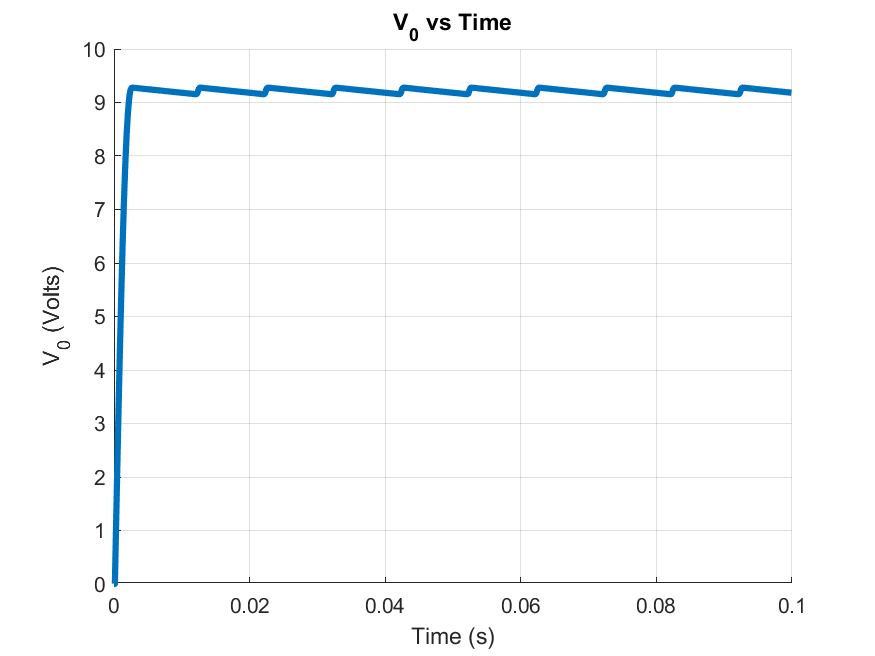
\includegraphics[width = 0.75\textwidth]{5.png}
\caption{Circuit schematic for the step 5}
\end{figure} 

%%%%%%%%%%%%%%%%%%%%%%   EXAMPLE IMAGE FROM PDF   %%%%%%%%%%%%%%%%%%%%%%%%%%%%%%%%
\begin{figure}[H] \centering{
	\includegraphics[scale=0.25]{2a_plot.pdf}}
	\caption{Experiment 2}
\end{figure}
%%%%%%%%%%%%%%%% Deneme Push